%! Author = julianmour
%! Date = 01/05/2023

\section{Preliminary Results}
We evaluated our preliminary approach on the Double-MNIST dataset, consisting of images showing two digits.
The multi-classifier's goal is to return the correct two digits. % from ten classes;
%$C = \{0, 1, \ldots,9\}$ (the 10 different digits), each image classified to two different classes (contains two different digits).
An example of an image is shown in Figure~\ref{fig:double-mnist-sample}. %, where the digit $4$ is the target object and the digit $9$ is the non-target object.
\begin{figure}
\centering
\begin{minipage}{.4\textwidth}
  \centering
  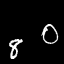
\includegraphics[width=0.6\linewidth]{108_80.png}
  \captionof{figure}{A Double-MNIST sample.}
   \label{fig:double-mnist-sample}
\end{minipage}%
\begin{minipage}{.6\textwidth}
  \centering
  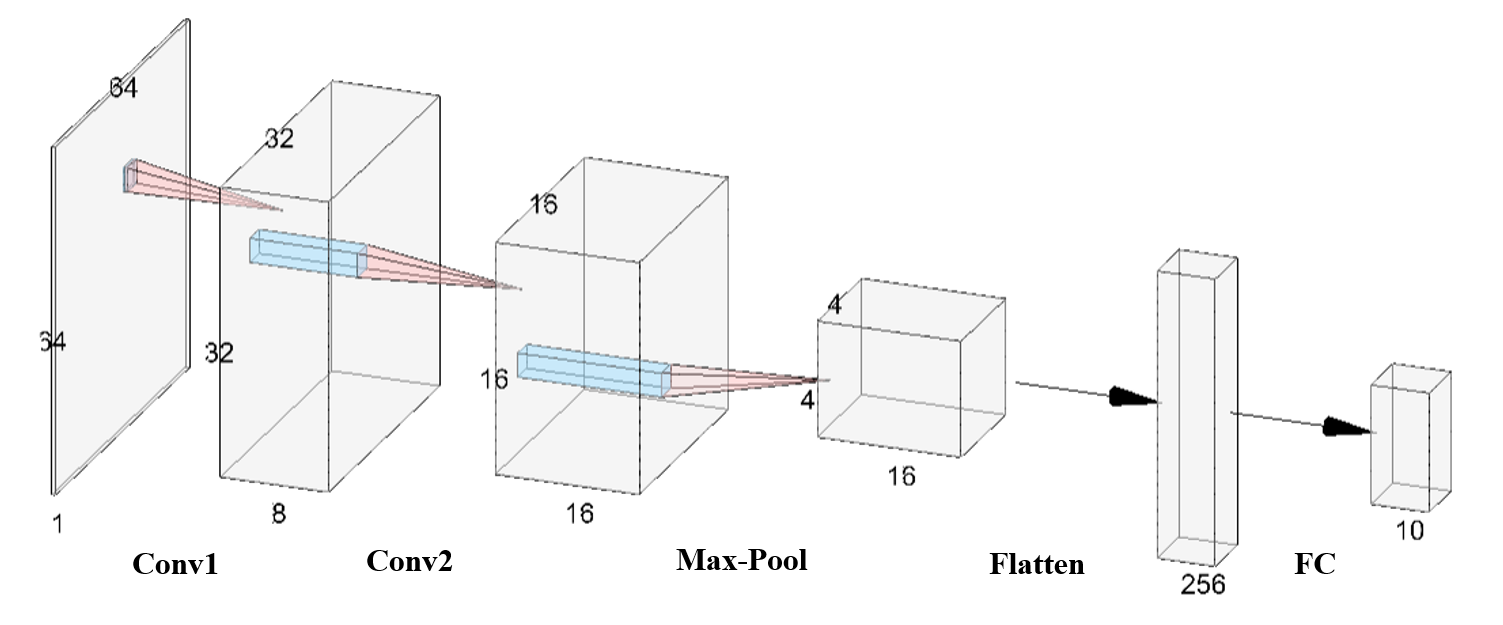
\includegraphics[width=1\linewidth]{arch_labeled.png}
  \captionof{figure}{The classifiers' architecture.}
  \label{fig:arch_labeled}
\end{minipage}
\end{figure}
We ran our algorithm on three different CNN multi-label DOUBLE-MNIST classifiers, all with the same architecture (shown in Figure~\ref{fig:arch_labeled}) but a different training procedure:

%\Dana{describe it and how many neurons}
%While the three of them solve the same classification problem, they differ in their training process:
\begin{itemize}
    \item Without defense. %- This network is trained regularly on the original DOUBLE-MNIST training dataset, without additional processing done to the training dataset.
      \item With an $L_0$ defense: This defense relies on the following data augmentation.
    Before forwarding a training sample to the network, we add random noise to the image in the form of a black rectangle.
        \item With an $L_{\infty}$ defense: Using the Projected Gradient Descent (PGD) defense~\cite{PGD}.
    This defense also involves training the model with adversarial examples, but unlike the $L_0$ defense, the added perturbations are a small value and can be anywhere in the input.
    %The PGD generated adversarial examples are achieved by trying to increase the model's loss function as much as possible.
    %Therefore, training the model with such adversarial examples should make the network more robust.
\end{itemize} 

To compare between the robustness of the models, we ran our algorithm on each of them, for 30 images. We run our algorithm twice, once for each cutting weights type (fixed and based on sensitivity). We measure the average neighborhood size defined as \Dana{complete the math computation}. We also measure that the average execution time for a single image, which is about \Dana{complete}.
Figure~\ref{fig:neighborhoods_average_size} shows the average neighborhood size for each model and each cutting weights type.
The result show that, as expected, the defended models are more robust and the $L_{\infty}$ defended model is the most robust.
This is expected because our attack model focuses on the $L_{\infty}$ norm.
 The results further show that using sensitivity weights as cutting weights enable our algorithm to synthesize larger robust neighborhoods.
%The average size of the neighborhoods returned by our program is presented in Figure~\ref{fig:neighborhoods_average_size}.
\begin{figure}
    \centering
    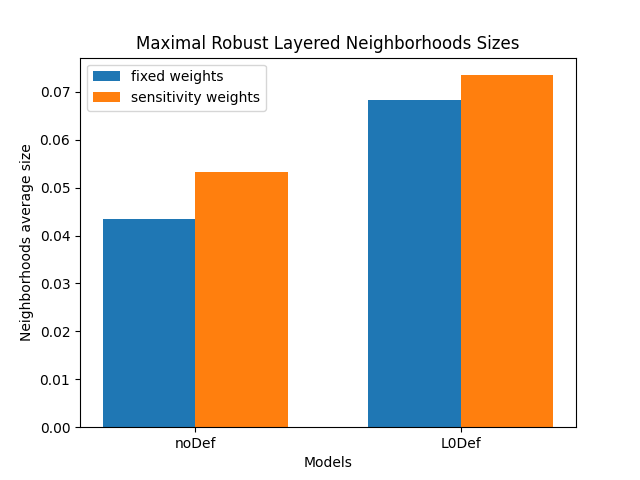
\includegraphics[width=0.7\textwidth]{neighborhoods_average_size.png}
    \caption{The average size of the synthesized neighborhoods.\Dana{remove the title "Maximal robust..."}}
    \label{fig:neighborhoods_average_size}
\end{figure}
%
  Figure~\ref{fig:No defense} demonstrates the difference between the types of the cutting weights. For a given image, the undefended classifier and a cutting weight type, we show the heat map corresponding to synthesized layered neighborhood. The heat maps show \Dana{complete}.
  Figure~\ref{fig:L0 defense} is similar but for the $L_0$ defended network. The heat maps show \Dana{complete}.
    \begin{figure}
         \centering
         \begin{subfigure}[b]{0.4\textwidth}
             \centering
             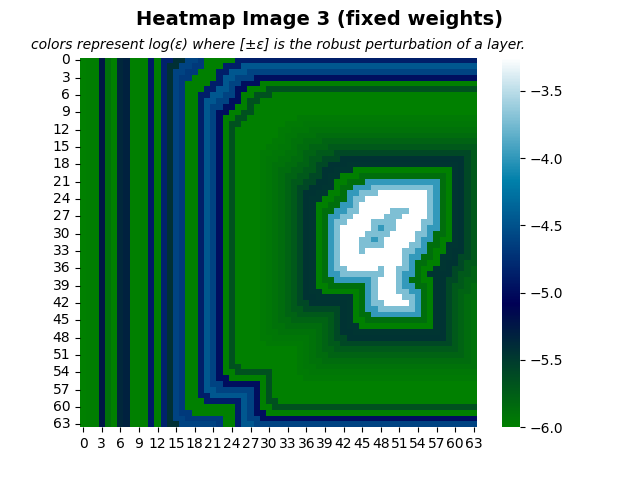
\includegraphics[width=\textwidth]{no_defense_fixed_weights.png}
             \caption{fixed weights}
             \label{sub-fig:No defense FW}
         \end{subfigure}
         \hfill
         \begin{subfigure}[b]{0.4\textwidth}
             \centering
             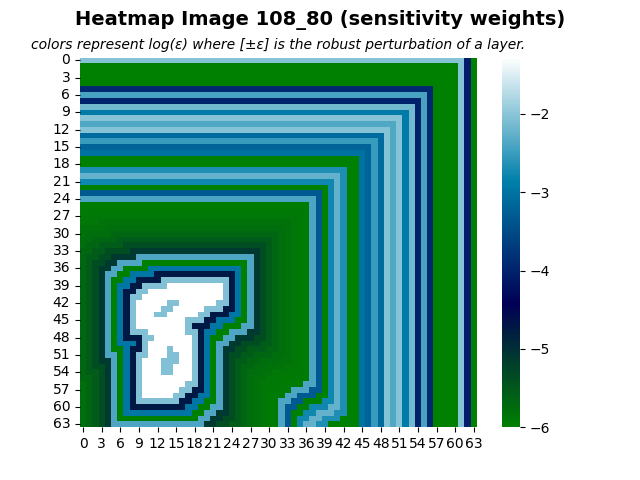
\includegraphics[width=\textwidth]{no_defense_sensitivity_weights.png}
             \caption{sensitivity weights}
             \label{sub-fig:No defense SW}
         \end{subfigure}
         \caption{No Defense}
         \label{fig:No defense}
     \end{figure}
    % In Figure~\ref{fig:L0 defense} we present results of our program ran on a classifier trained with $L_0$ defense, and a single image, as a heatmap representing the epsilons per each layer.
    \begin{figure}
         \centering
         \begin{subfigure}[b]{0.4\textwidth}
             \centering
             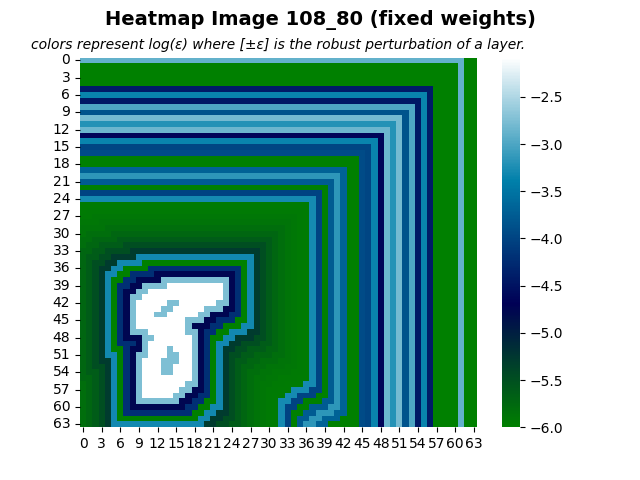
\includegraphics[width=\textwidth]{l0_defense_fixed_weights.png}
             \caption{fixed weights}
             \label{sub-fig:L0 defense FW}
         \end{subfigure}
         \hfill
         \begin{subfigure}[b]{0.4\textwidth}
             \centering
             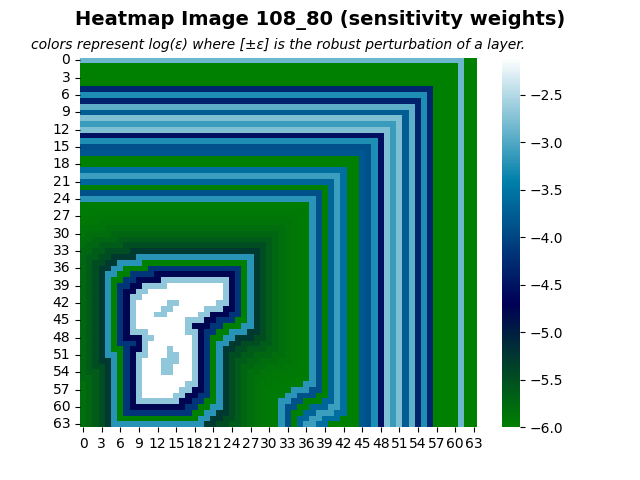
\includegraphics[width=\textwidth]{l0_defense_sensitivity_weights.png}
             \caption{sensitivity weights}
             \label{sub-fig:L0 defense SW}
         \end{subfigure}
         \caption{$L_0$ Defense}
         \label{fig:L0 defense}
    \end{figure}
